\documentclass[10pt]{beamer}
\usetheme[
%%% options passed to the outer theme
%    hidetitle,           % hide the (short) title in the sidebar
%    hideauthor,          % hide the (short) author in the sidebar
%    hideinstitute,       % hide the (short) institute in the bottom of the sidebar
%    shownavsym,          % show the navigation symbols
%    width=2cm,           % width of the sidebar (default is 2 cm)
%    hideothersubsections,% hide all subsections but the subsections in the current section
%    hideallsubsections,  % hide all subsections
%    right                % right of left position of sidebar (default is right)
  ]{Aalborg}

\definecolor{aaublue}{RGB}{33,26,82}
\definecolor{aaugrey}{RGB}{84,97,110}

% If you want to change the colors of the various elements in the theme, edit and uncomment the following lines
% Change the bar and sidebar colors:
\setbeamercolor{Aalborg}{fg=aaublue!10,bg=aaugrey!60}
%\setbeamercolor{sidebar}{bg=blue!74}
% Change the color of the structural elements:
\setbeamercolor{structure}{fg=aaublue}
 \setbeamercolor{subtitle}{fg=aaugrey}
% Change the frame title text color:
\setbeamercolor{frametitle}{fg=aaublue}
% Change the normal text color background:
%\setbeamercolor{normal text}{bg=aaugrey!10}
% ... and you can of course change a lot more - see the beamer user manual.
\usebackgroundtemplate{
\includegraphics[width=\paperwidth]{img/background}}

\usepackage[utf8]{inputenc}
\usepackage[english]{babel}
\usepackage[T1]{fontenc}
\DeclareUnicodeCharacter{00A0}{~} % Fixes the "! Package inputenc Error: Unicode char \u8:  not set up for use with LaTeX."
% ... or whatever. Note that the encoding and the font should match. If T1
% does not look nice, try deleting the line with the fontenc.
\usepackage{lmodern} %optional

% colored hyperlinks
\newcommand{\chref}[2]{%
  \href{#1}{{\usebeamercolor[bg]{Aalborg}#2}}
}

\title[Centralized State Estimation\\ of Distributed Maritime Autonomous Surface Oceanographers]% optional, use only with long paper titles
{Centralized State Estimation of Distributed Maritime Autonomous Surface Oceanographers}

%\subtitle[v.\ 0.1.1] %optional
%{v.\ 0.1.1}

\author[12gr730]{% optionally input the group number, use only with lots of authors
  Attila Fodor \and Rasmus L. Christensen \and Frederik Juul \and Tudor Muresan \and Nick \O stergaard\\
  {{\tt \{afodor12,ralch,fjuul,tmures12,nickoe\}@es.aau.dk}}
}
% - Give the names in the same order as they appear in the paper.
% - Use the \inst{?} command only if the authors have different
%   affiliation. See the beamer manual for an example

%specify some optional logos
\pgfdeclareimage[height=1.2cm]{mainlogo}{aau_logo.pdf} % placed in the upper left/right corner
\logo{\pgfuseimage{mainlogo}}

\pgfdeclareimage[height=0.75cm]{logo2}{tu-logo} % placed in the lower left/right corner if the \pgfuseimage{logo2} command is uncommented in the \institute command below

\institute[
%  {\pgfuseimage{logo2}}\\ %insert a company or department logo
  Dept.\ of Electronic Systems,\\
  Aalborg University,\\
  Denmark
] % optional - is placed in the bottom of the sidebar on every slide
{%
  Department of Electronic Systems,\\
  Aalborg University,\\
  Denmark
  
  %there must be an empty line above this line - otherwise some unwanted space is added between the university and the country (I do not know why;( )
}
\date{\today}

\begin{document}
% the titlepage
\begin{frame}[plain] % the plain option removes the sidebar and header from the title page
  \titlepage
\end{frame}
%%%%%%%%%%%%%%%%

% TOC
\begin{frame}{Agenda}{}
\tableofcontents
\end{frame}
%%%%%%%%%%%%%%%%
\section{Introduction}
\begin{frame}{Introduction}{Purpose}
  \begin{itemize}
  	\item<1-> Little to no research are currently devoted to maritime autonomous crafts.
    \item<2-> During the 2012 Fukushima accident in Japan, no measurements of the spread of radioactivity was available in the coastal zones, thus relying only on estimates. 
    \item<3-> The coastal area around Greenland has no up-to-date baymethric maps available, and with the growing interest in Greenland (both industrially and commercially) this poses a threat to the ships going in and out of the fjords.
  \end{itemize}
\end{frame}
%%%%%%%%%%%%%%%%
\begin{frame}{Introduction}{Problem Description}
Empty frame
\end{frame}

%%%%%%%%%%%%%%%%
\section{Development}
\subsection{AAUSHIP.01}
\begin{frame}{Development}{AAUSHIP.01}
\begin{itemize}
	\item<1-> The ship is designed as a non-planing deplacement craft (eg. like freight ships).
	\item<2-> Developed using rapid prototyping techniques.
	\item<3-> Developed in Rhinoceros\texttrademark using a lofting techniques.
	\item<4-> Printed on a 3D printer.
	\item<5-> Examined and the process iterated.
	\item<6-> Vaccumformed by DD-plast in Randers and assembled in the machine shop at Aalborg University.
\end{itemize}
\end{frame}

%%%%%%%%%%%%%%%%
\begin{frame}{Development}{AAUSHIP.01 Hull}
\begin{figure}
	\begin{center}
		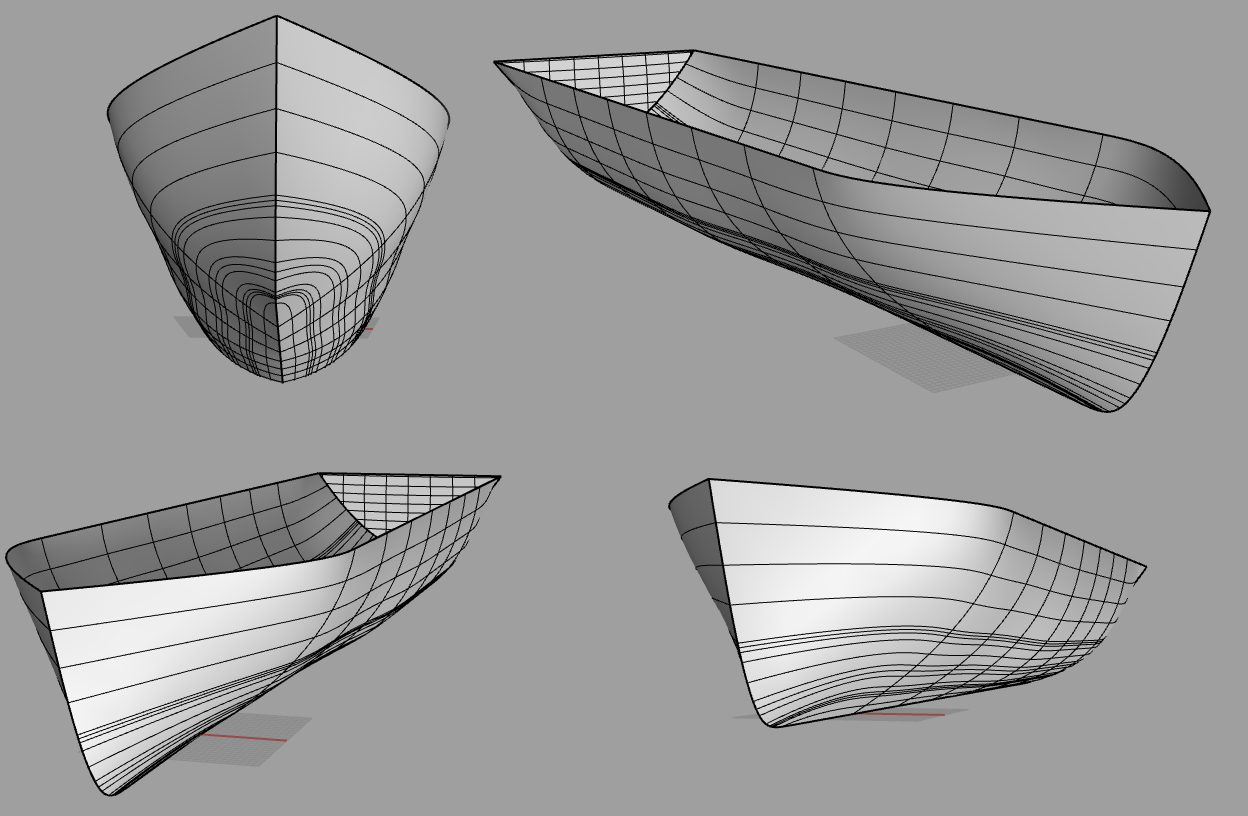
\includegraphics[width=8.2cm]{img/rendermontage}
		\label{fig:render}
	\end{center}
\end{figure}
\end{frame}

%%%%%%%%%%%%%%%%
\begin{frame}{Development}{AAUSHIP.01 Hull}
\begin{figure}
	\begin{center}
		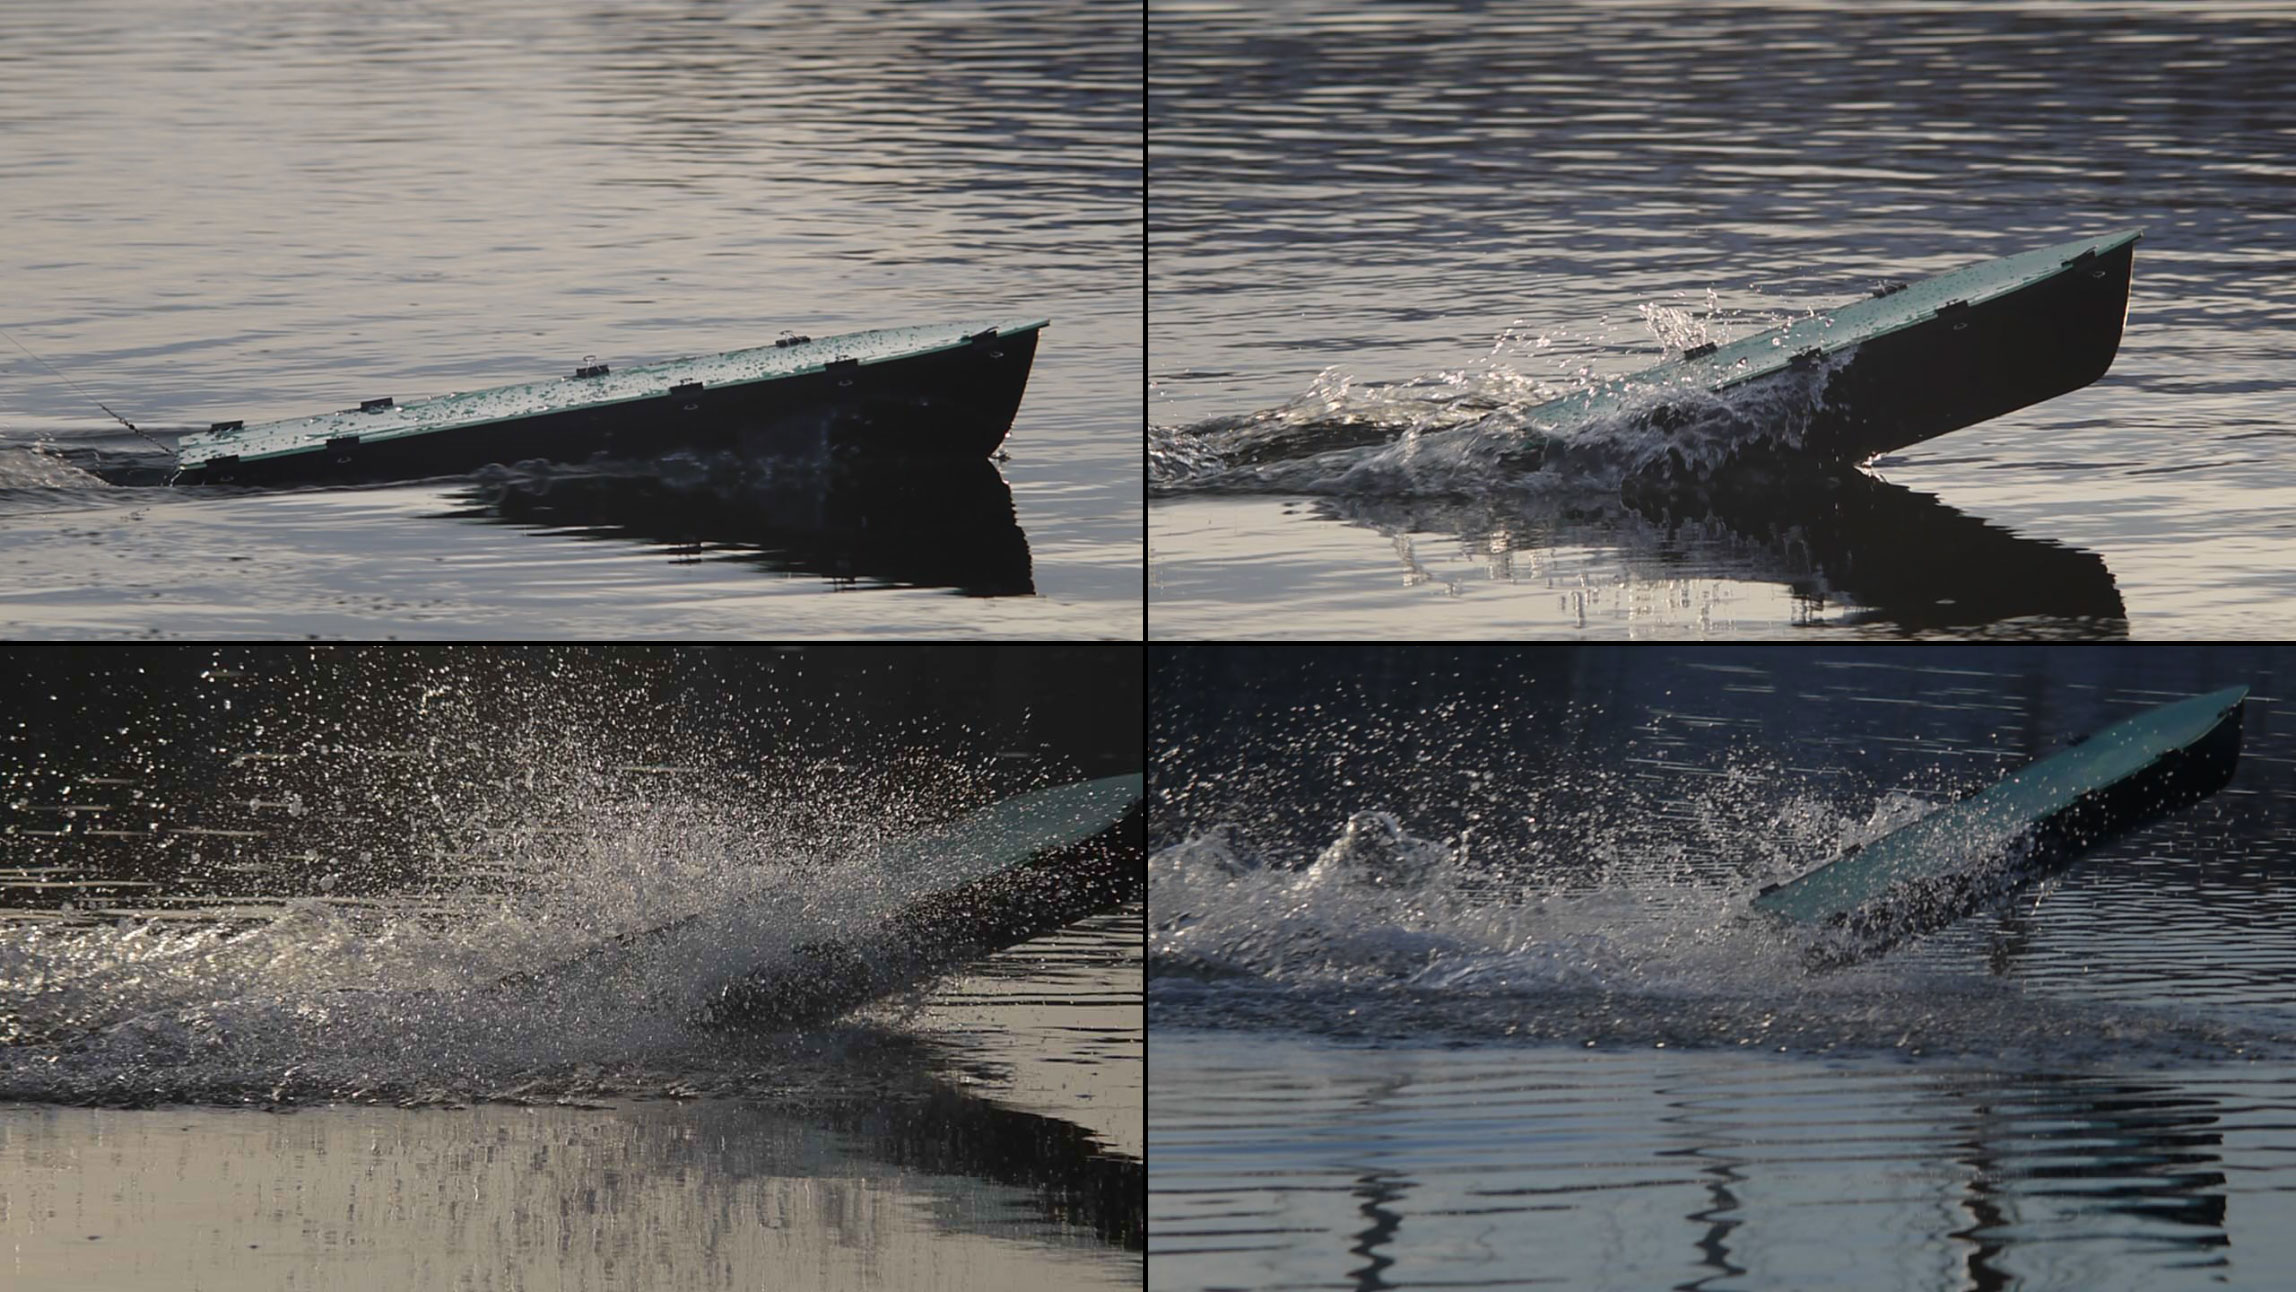
\includegraphics[width=8.2cm]{img/VerticalJumpingTele}
		\label{fig:jumping}
	\end{center}
\end{figure}
\end{frame}

%%%%%%%%%%%%%%%%
\subsection{Development}
\begin{frame}{Development}{Hardware}
\begin{itemize}
	\item Fitted with 2 x 1200W engines (totally producing around 3 HP at full thrust).
	\item Fitted with 6 x 3200mAh batteries (results in a mission time of around 5 hours).
	\item 2 counter rotating 60mm propellers.
	\item Inertial Measurement Unit.
	\item Global Positioning System.
	\item A 20mW 19.2 kbps radio link @ 470 MHz
	\item Arduino Mega with a custom made shield board mounted.
    \item Retrofitted with a hydrofoil to reduce the wake and pitch of the ship.
\end{itemize}
\end{frame}
%%%%%%%%%%%%%%%%
\begin{frame}{Development}{Protocol}
The designed protocol is given as:
\end{frame}

%%%%%%%%%%%%%%%%
\begin{frame}{Development}{Distributed Control}
As the protocol takes care of packet verification, the channel can be estimated by a bernoulli variable, with outcomes of a received package either a succes or a failure.
\begin{figure}
	\begin{center}
		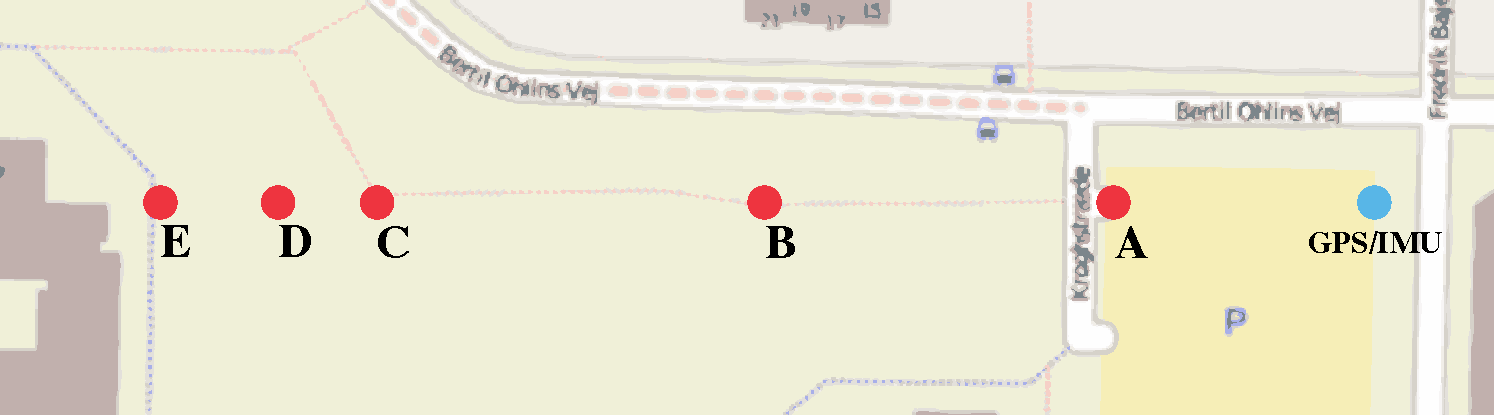
\includegraphics[width=8.2cm]{img/measpoint}
		\label{fig:measpoint}
	\end{center}
\end{figure}
The measurements make for the following distribution of the GPS with a distance of 189 metres:
\begin{align}
\lambda_\text{gps,E} = \left\{ 
  \begin{array}{l l}
    0.8643 & \quad \text{for $\lambda$ = 1}\\
    0.1357 & \quad \text{for $\lambda$ = 0}
  \end{array} \right.
\end{align}
And for the IMU also at 189 metres.
\begin{align}
\lambda_\text{imu,E} = \left\{ 
  \begin{array}{l l}
    0.8689 & \quad \text{for $\lambda$ = 1}\\
    0.1311 & \quad \text{for $\lambda$ = 0}
  \end{array} \right.
\end{align}
\end{frame}

%%%%%%%%%%%%%%%%
\begin{frame}{Development}{Kalman Filter}
The derivation of the Kalman filter is based around the position being equal to the last position, the change due to velocity and the change due to acceleration:
\begin{align}
x[n] &= x[n-1] + \dot{x}[n-1]\cdot ts + \ddot{x}[n-1]\cdot \frac{ts^2}{2}\\
\dot{x}[n] &= \dot{x}[n-1] + \ddot{x}[n-1] \cdot ts\\
\ddot{x}[n] &= -\beta \cdot \dot{x}[n-1] + \ddot{x}[n]
\end{align}
Which can be put on matrix form:
\begin{align}
\begin{bmatrix}
x[n]\\
\dot{x}[n]\\
\ddot{x}[n]
\end{bmatrix} = \begin{bmatrix}
1 & ts & \frac{ts^2}{2}\\
0 & 1 & ts\\
0 & -\beta & 0
\end{bmatrix}\begin{bmatrix}
x[n-1]\\
\dot{x}[n-1]\\
\ddot{x}[n-1]
\end{bmatrix}
\end{align}
This goes for the $y$-axis and the rotation about the $z$-axis as well.
\end{frame}

\chapter{Control}
\label{chap:control}

\section{Overview of the control system}
This is an overview of the information flow for control in regard to the rest of the system containing, sensors, \ac{LLI} and \ac{HLI}.

\begin{figure}[htbp]
	\centering
	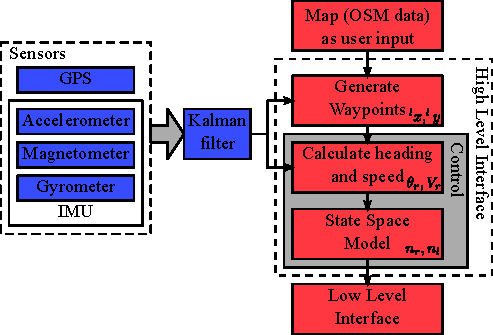
\includegraphics[width=\textwidth]{img/vessel-block-overview}
	\caption{Overview of control information flow in regard to the subsystems. The blue part indicates information that is not fetched directly to the control part, it is electrically connected to the \ac{LLI} whilst being forwarded to the \ac{HLI}.}
	\label{fig:vessel-block-overview}
\end{figure}

\todo{Illustrate on figure~\vref{fig:vessel-block-overview} where RF comms is or maybe that should be on the block overvieww diagram without regard to contorl abstraction}



In the First Stage the required heading of the ship is calculated that keeps the course closest to the planned waypoint.

In order to efficiently and accurately navigate along the path, a set of Sub-Waypoints is calculated for each route between two Waypoints. The main control strategy of the first path is to navigate through all of these SWPs in a predefined order, one by one. (Navigation Figure) The heading of the ship is defined in NED coordinate system. The required heading is determined by the law of Cosines, based on the Position of the Ship and the Position of the next Sub-Waypoint.
\begin{center}
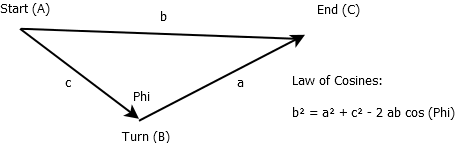
\includegraphics[scale = 0.4]{img/ControlStrategyFigures/Law_of_Cosines.png}
\end{center}
Problems rise and corrections are necessary, if the heading of the ship $\theta$ is $\theta < -\pi$ or $\theta < \pi$. The heading of the ship is calculated based on the Gyro sensor and the heading can have any value in the form of: $$\theta = [-{\pi} ; \pi ] \pm 2*k*\pi$$. Before invoking the control procedure, all of the heading angles must be transformed into the $[-\pi ; \pi]$ interval.
This procedure causes a possible error though.

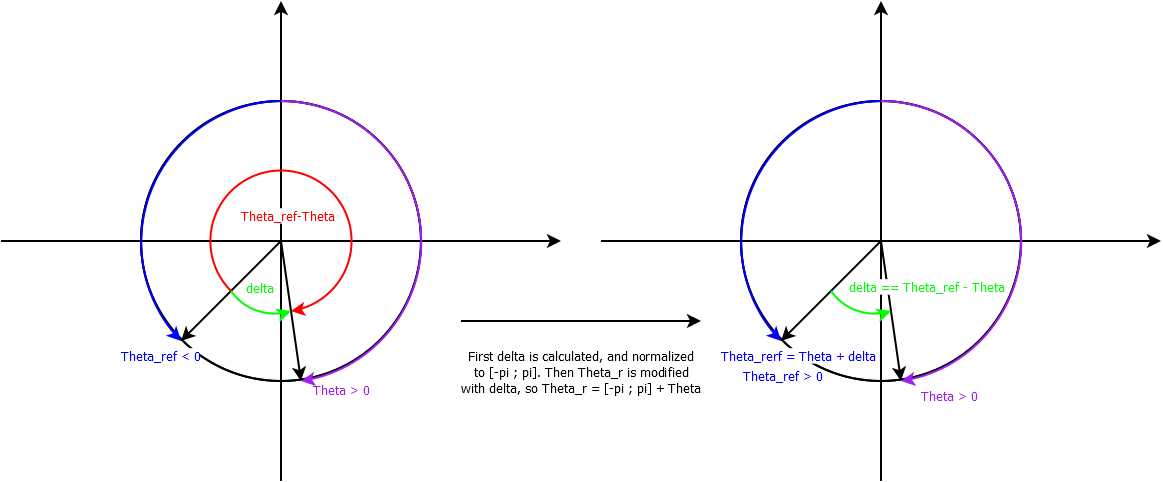
\includegraphics[width=\textwidth]{img/ControlStrategyFigures/Headings.png}

The required heading or the heading of the ship must be transformed into a different representation, where $$|\theta_{r}-\theta| < \pi$$. To keep a consistent heading representation, first the deviation angle $$\theta = \pi_{r}-\pi$$ is calculated, than transformed to the $[-\pi;\pi]$ interval and finally, with $\delta$ we can transform $\theta_{r}$ to $$\theta_{r}(\theta) = \theta + \delta$$.
If the conditions above are met, $\theta$ and $\theta_r(\theta)$ will always yield values that result in correct controller output.

\subsection{Subwaypoint Validity}

The overall navigation can be improved, if the Target SWPs are considered ''reached´´ in a certain distance. Optimally this distance (Validity distance) should be somewhat longer than the minimum turning radius of the ship ($R_{min}$). If it is shorter, the ship might not be able to reach the SWP, if it is way longer, the ship will divert from its course in turns.

%1. what is it
\todo{description}

%2. why are we using it


The reason for which the State Space representation was chosen is because it is a very simple, yet powerful way of modeling linear systems, allowing us to adjust and manipulate its dynamics in a very wide range of situations. 

%3. what are we using from it

\subsection{Linearizing the outputs}

Using Newton's second law of motion for forward  and rotational movement (F = m * A; T = I * W'), we can easily see that the inputs to our system will be F and T representing the forward force and the torque produced by the motors. It is worth mentioning that, since there are two propellers rotating in opposite directions, a torque that would induce a rotation around Z axis passing through the boat's center of mass only if the two propellers are rotating at different speeds.

These two rotational speeds N1 and N2 were initially included in the state space model as inputs to the system, as they could be controlled directly via a PWM pulse. This though proved to complicate matters because the relationship between the speeds of the propellers N1 and N2 and the force F and torque T generating accelerations is not a linear one. Because of this, our system would not be linear and would be beyond the scope of this project. 

\todo{insert formulas for [F, T] -> [n1, n2] transformation here}

In order to prevent this from happening, the state space model was updated to only calculate the force T and torque T necessary for driving and turning the ship, and this would keep our system linear. in order to transform from [T, F] to [N1, N2], another module was introduced in the system which would implement this non-linear function. 

This is a better solution anyway because if the state space model only outputs T and F, then it could be used for some other ship configurations, without modifications to the model, only to the module that translates the force and torque to N1 and N2. This, for example, can allow us to change the size of the propellers or their positions.

\subsection{Linearizing the drag forces}
\label{sect:Linearizing drag forces}

The drag forces acting on the bow of the ship while it's moving through the water are influenced by the area of the hull that is below water depth in the direction of movement, the density of the water, a drag constant $ C_{D} $ , and the square of the ship's speed components $ v_{x} $ and $ v_{y} $. 

A worthy note is the fact that the drag coefficient $ C_{D} $ will have two values depending on the direction of the ship's movement. When moving forward in the x direction, the coefficient $ C_{D}x $ will be approximated for a triangular shape, which is the closest simple shape that we have values for. For lateral movement in the y direction, $ C_{D}y $is given for a square box. These approximations should not present a problem in the operation of our control system as the errors ca easily be corrected and adjusted for by a good controller.

\[ D_{x}(v_{x}) = \frac{C_{Dx}\cdot\rho_{water}\cdot A_{front}\cdot v_{x}^{2}}{2} \]
\[ D_{y}(v_{y}) = \frac{C_{Dy}\cdot\rho_{water}\cdot A_{side}\cdot  v_{y}^{2}}{2} \]

Where $ D_{x}(v_{x}) $ and $ D_{y}(v_{y})$ are the drag forces dependent on the forward and lateral speeds respectively, $ \rho_{water} $ is the density of the water, $ A_{front} $ is the frontal area of the hull and $ A_{side} $ is the lateral area. 

The drag torque that is produced by the drag force acting on the hull of the ship, as the ship rotates through the water is dependent on the square of the angular velocity $ \omega $:

\[ \tau(\omega) = \frac{C_{D} \cdot \rho_{water} \cdot d \cdot (r_{f}^{4} + r_{b}^{4}) \cdot \omega^{2}}{8} \]

Where $ \tau(\omega) $ is the torque generated by the angular speed $ \omega $, $ d  $ is the depth of the ship that is submerged in water, $ r_{f} $ and $ r_{b} $ are the radii of the ship from the center of mass towards the front and back end, respectively.

These forces are obviously non-linear and thus cannot be integrated into the linear Kalman filter or State Space Model. Because we will usually use a constant speed it is feasible to linearize these forces for that value and not have big errors. The angular drag torque can also be linearized around a mean turning speed because the radii of the corners of the paths are also constant.

Approximation of the drag forces around the points of interest $v_{l} $ and $\omega_{l}$ is done using the first order term of the Taylor expansion:

\[ y_{l}(x) = f(a) + f'(a)(x-a) \]

Where $y = f(x)$ is the function we want to linearize around a value of interest $a$. Applying this formula to our situation yields:

\[ Dx_{l}(v_{x}) = \frac{C_{D}x\cdot\rho_{water}\cdot A_{front}\cdot v_{l}^{2}}{2} + (C_{D}x\cdot\rho_{water}\cdot A_{front})\cdot (v_{x}-v_{l}) \]

\[ Dy_{l}(v_{y}) = \frac{C_{Dy}\cdot\rho_{water}\cdot A_{side}\cdot v_{l}^{2}}{2} + (C_{D}y\cdot\rho_{water}\cdot A_{side})\cdot (v_{y}-v_{l}) \]

\[ \tau_{l}(\omega) = \frac{C_{D}y \cdot \rho_{water} \cdot d \cdot (r_{f}^{4} + r_{b}^{4}) \cdot \omega_{l}^{2}}{8} + \frac{C_{D}y \cdot \rho_{water} \cdot d \cdot (r_{f}^{4} + r_{b}^{4}) \cdot \omega_{l}}{4} \cdot (\omega - \omega_{l}) \] 

\begin{figure}[htbp]
	\centering
	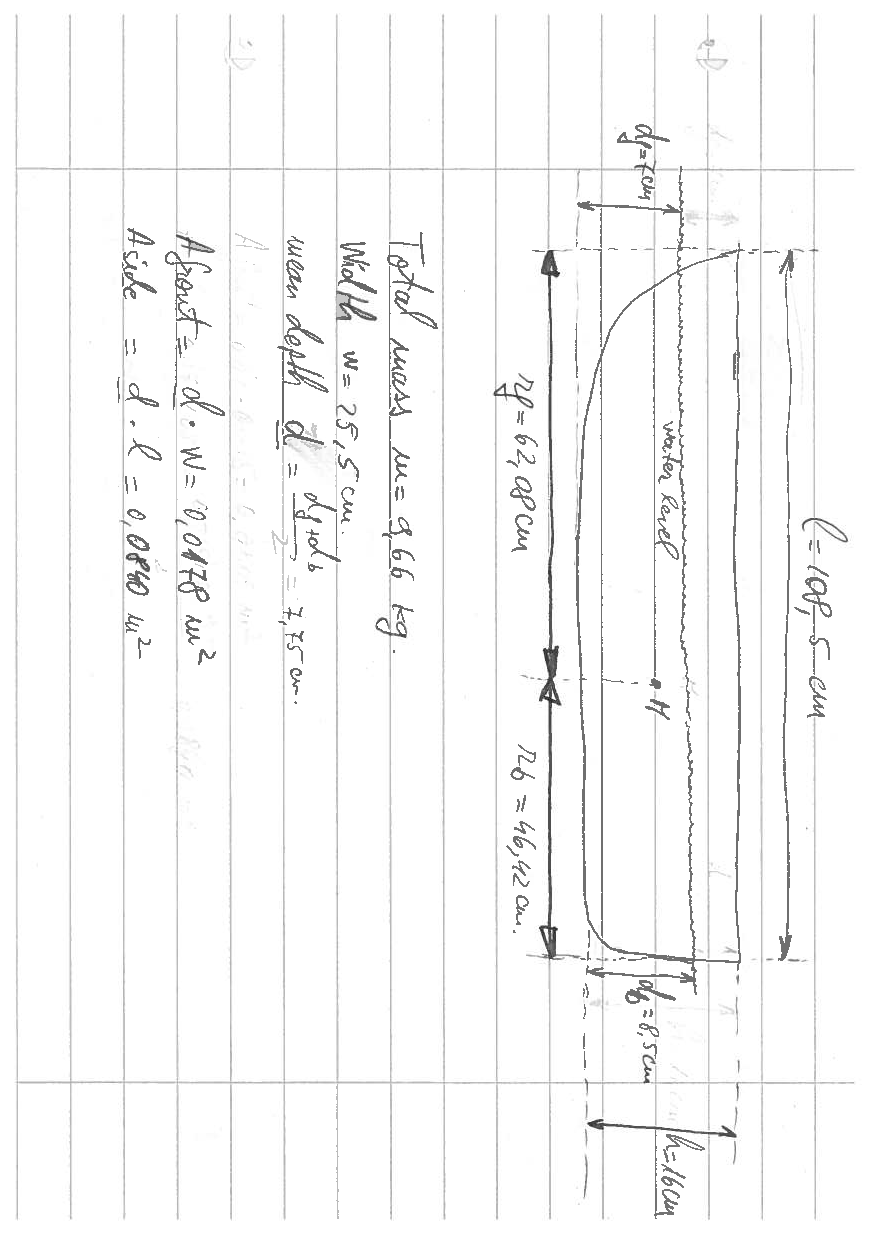
\includegraphics[width=\textwidth, trim=1.8cm 0cm 0cm 2cm, clip = true, angle = 90, width=\textwidth]{img/ship_sizes}
	\caption{Sketch of ship sizes as measured after the maiden voyage}
	\label{fig:ship_sizes}
\end{figure}

Given \vref{fig:ship_sizes}
 $ v_{l} = 1m/s $ ,
 $ \omega_{l} = 1 s ^{-1} $ ,
 $ C_{D}x = 0.5 $ (triangle) ,
 $ C_{D}y = 1 $ (box) ,
 $ \rho = 1000 kg/m ^{2} $,
 $ A_{front} = 0.0178 m^{2} $,
 $ A_{side} = 0.0840 m ^{2} $,
 $ d = 0.0775 m $,
 $ r_{f} = 0.6208 m $,
 $ r_{b} = 0.4642 m $,
the linearized formulas for the drag forces can be computed to be:


\begin{align}
 Dx_{l}(v) &= -4.45 + 8.9 \cdot v_{x} \\
 Dy_{l}(v) &= -42 + 84 \cdot v_{y} \\
 \tau_{l}(\omega) &= -1.88 + 3.77 \cdot \omega
\end{align}

From which we can identify the coefficients that correspond tot the linear relation $ y_{l}(x) = \alpha + \beta \cdot x $:\\
\begin{minipage}{0.3\linewidth}
\[ \alpha_{x} = -4.45 \] 
\[ \beta_{x} = 8.9 \]
\end{minipage}
\begin{minipage}{0.3\linewidth}
\[ \alpha_{y} = -42 \] 
\[ \beta_{y} = 84 \]
\end{minipage}
\begin{minipage}{0.3\linewidth}
\[ \alpha_{\omega} = -1.88 \]
\[ \beta_{\omega} = 3.77 \]
\end{minipage}


\subsection{Choosing the right states}

The variables we chose to be the states in our model are the speed of the ship in the forward direction in the ship frame $v$, the angular position of the ship's x axis relative to true North $\theta$ and the angular speed $\omega$.\\
\[\begin{cases}
F - F_{D} = m \cdot \dot{v}\\
T - T_{D} = I \cdot \dot{\omega}\\
\end{cases}\]

Where $ F $ and $ T $ are the force and torque produced by the propellers, $ F_{D} $ and $ T_{D} $ are the force and torque caused by water drag, $ m $ is the mass of the ship, $ I $ is the moment of inertia, $ \dot{v} $  and $ \dot{\omega} $ are forward and angular acceleration respectively.

The linearized drag force and torque from \ref{sect:Linearizing drag forces} can be substituted in these equations:
\begin{align}
 \dot{v} &= - \frac{\beta_{x} \cdot v}{m} + \frac{F}{m}\\
 \dot{\omega} &= - \frac{\beta_{y} \cdot \omega}{I} + \frac{T}{I}\\
 \dot{\theta} &= \omega
\end{align}

Note that we have also dropped the $ \alpha $ term of the equations because we're currently only interested in the dynamic behavior of the system. The $ \alpha $ offset will be compensated for when removing the steady state error. Consequently, these relations can be rewritten in a matrix notation as follows:
\[
\dot{
	\begin{bmatrix}
	 v\\
	 \theta\\
	 \omega
	\end{bmatrix}
}
=
\begin{bmatrix}
 -\frac{\beta_{x}}{m} & 0 & 0\\
 0 & 0 & 1\\
 0 & 0 & - \frac{\beta_{y}}{I}\\
\end{bmatrix}
\cdot
\begin{bmatrix}
v\\
\theta\\
\omega
\end{bmatrix}
+
\begin{bmatrix}
\frac{1}{m} & 0\\
0 & 0\\
0 & \frac{1}{I}\\
\end{bmatrix}
\cdot
\begin{bmatrix}
F\\
T
\end{bmatrix}
\]

This corresponds to the State Space Model equation:
\[\dot{X} = AX + BU\]

Since the output matrix we need is $ Y = \begin{bmatrix}v \\ \theta \end{bmatrix} $, the output equation
\[Y = CX + DU\]
becomes:
\[\begin{bmatrix}v \\ \theta \end{bmatrix}
 = 
\begin{bmatrix}
1 & 0\\
0 & 1\\
0 & 0
\end{bmatrix}
\cdot
\begin{bmatrix}
v\\
\theta\\
\omega
\end{bmatrix}
\]

So the system matrices are:
\[
A =\begin{bmatrix}
 -\frac{\beta_{x}}{m} & 0 & 0\\
 0 & 0 & 1\\
 0 & 0 & - \frac{\beta_{y}}{I}\\
\end{bmatrix}\\
B = \begin{bmatrix}
\frac{1}{m} & 0\\
0 & 0\\
0 & \frac{1}{I}\\
\end{bmatrix}\\
C = 
\begin{bmatrix}
1 & 0\\
0 & 1\\
0 & 0
\end{bmatrix}\\
D = 0
\]

\subsection{Discretizing for use with a particular timestep}

The system described so far is continuous and needs to be discretized before implementation in a computer algorithm, so we use the function c2d from MATLAB and the time step Ts in order to do this. \todo{explain more about c2d or what we will eventually use}

\subsection{Pole assignment}

For assigning poles, we use the lqr function implemented in MATLAB. This calculates the gain matrix $ F $ by minimizing the quadratic cost function:\todo{taken from here http://www.mathworks.se/help/control/ref/lqr.html}
\[
J(u)=\sum_{0}^{\inf} \{x^{T}Qx+u^{T}Ru+2x^{T}Nu\}
\]


\subsection{Reference gain}

A reference gain is calculated and implemented in order to counter the steady state error. This is calculated using the formula $ N = Nu+FNx $ \todo{insert refference to feedback book, page 470}, where:
\[
\begin{bmatrix}
Nx\\
Nu
\end{bmatrix}
=
\begin{bmatrix}
A & B\\
C & D
\end{bmatrix}^{-1}
\!
\cdot
\begin{bmatrix}
0\\
I
\end{bmatrix}
\]
\todo{Why we chose a lot of states in the beginning, and then were left with just a few?}

%%%%%%%%%%%%%%%%
\section{Modeling}
\subsection{Engine model}
\begin{frame}{Modeling}{Thrust/Torque Model}
The thrust generated by the engines are modeled using equation \ref{eq:thrust} which is a function of the RPS of the propellers:
\begin{align}
F_\text{stbd,port} = \rho \cdot K_\text{T} \cdot D^4 \cdot |n_\text{stbd,port}| \cdot n_\text{stbd,port}
\label{eq:thrust}
\end{align}
As the engines are mounted on the starboard and port side the total thrust forward is a sum of the two engines $F_\text{total} = F_\text{stbd.} + F_\text{port}$ and the difference between them generates a torque around the centre of rotation
\begin{align}
\tau = (F_\text{stbd.} - F_\text{port}) \cdot l
\end{align}
Where $l$ denotes the distance from the centre of rotation to the top of the propellers.
\end{frame}

%%%%%%%%%%%%%%%%
\begin{frame}{Modeling}{Thrust/Torque Model}
Using Newtons 2nd law, the force and torque can be converted to an acceleration and an angular acceleration:
\begin{align}
\ddot{x} = \frac{F_\text{total}}{m} \quad \ddot{\theta} = \frac{\tau}{I}
\end{align}
Thus allowing for the input $\mathbf{u}$ to the system to be given as:
\begin{align}
\mathbf{u} = \begin{bmatrix}
F_\text{total} & \tau
\end{bmatrix}^T
\end{align}
And the $\mathbf{B}$ is given as the conversion from the force and torque to an acceleration and an angular acceleration respectively.
\begin{align}
\mathbf{B} = \begin{bmatrix}
\frac{1}{m} & \frac{1}{I}
\end{bmatrix}^T
\end{align}
\end{frame}

%%%%%%%%%%%%%%%%
\subsection{Ship Model}
\begin{frame}{Modeling}{System Dynamics}
The Dynamics of the system are given by the drag the ship experiences when moving through the water. The drag is given as:
\begin{align}
F_\text{Drag}(\dot{x},\dot{y}) = \frac{1}{2} \cdot \rho \cdot C_\text{D} \cdot \dot{x}^2 \cdot A 
\end{align}
The formula changes when the ship is turning, as the drag then is converted into a torque - which is defined as:
\begin{align}
\tau_\text{Drag}(\omega) = \frac{1}{2} \cdot \rho \cdot C_\text{D} \cdot (d \cdot (r_f^4 + r_b^4)) \cdot \omega^2
\end{align}
The above can be put an matrix form as:
\begin{align}
\mathbf{A}\mathbf{x} = \begin{bmatrix}
-\beta_X & 0 & 0\\
0 & -\beta_Y & 0\\
0 & 0 & -\beta_\omega
\end{bmatrix}\begin{bmatrix}
\dot{x}\\
\dot{y}\\
\dot{\theta}
\end{bmatrix}
\end{align}
\end{frame}

%%%%%%%%%%%%%%%%
\begin{frame}{Modeling}{System Dynamics}
As the motion in the $y$-direction is uncontrollable, and the thing to be controlled is the velocity and the angle, the combined system becomes:
\begin{align}
\dot{\mathbf{x}} &= \mathbf{A}\mathbf{x} + \mathbf{B}\mathbf{u}\\
\begin{bmatrix}
\ddot{x}\\
\dot{\theta}\\
\dot{\omega}
\end{bmatrix} &= \begin{bmatrix}
\frac{-\beta_x}{m} & 0 & 0\\
0 & 0 & 1\\
0 & 0 & \frac{-\beta_\omega}{I}
\end{bmatrix}\begin{bmatrix}
\dot{x}\\
\theta\\
\omega
\end{bmatrix} + \begin{bmatrix}
\frac{1}{m} & 0\\
0 & 0\\
0 & \frac{1}{I}
\end{bmatrix}\begin{bmatrix}
F_\text{total}\\
\tau
\end{bmatrix}
\end{align}
And the output of the system $\mathbf{y}$ becomes:
\begin{align}
\mathbf{y} &= \mathbf{C}\mathbf{x} + D\mathbf{u}\\
\begin{bmatrix}
\dot{x}\\
\theta\\
\end{bmatrix} &= \begin{bmatrix}
 1 & 0 & 0\\
 0 & 1 & 0
\end{bmatrix}\begin{bmatrix}
\dot{x}\\
\theta\\
\omega
\end{bmatrix} + \mathbf{0}\begin{bmatrix}
F_\text{total}\\
\tau
\end{bmatrix}
\end{align}
\end{frame}


%%%%%%%%%%%%%%%%
\section{Control}
\subsection{State Space Controller}
\begin{frame}{Control}{State Space Control}
\begin{itemize}
	\item Optimal Control
	\item Reference Tracking
\end{itemize}
\end{frame}

%%%%%%%%%%%%%%%%
\subsection{Implementation}
\begin{frame}{Control}{Implementation}
Empty Frame
\end{frame}

%%%%%%%%%%%%%%%%
\section{Test Results}
\subsection{Kalman Filter}
\begin{frame}{Test Results}{Kalman Filter}
Empty Frame
\end{frame}

%%%%%%%%%%%%%%%%
\subsection{Open water tests}
\begin{frame}{Test Results}{Maiden Voyage}
Empty Frame
\end{frame}

%%%%%%%%%%%%%%%%
\begin{frame}{Test Results}{Autonomous Sailing}
Empty Frame
\end{frame}


%%%%%%%%%%%%%%%%

\end{document}
